%DLA (Document) layout analysis
%ATR Automatic Text Recognition
%TAL:


%Template v.1.0: Taylor Arnold and Simon Gabay, december 2025
% CECI EST UN FICHIER DE MODÈLE LATEX POUR LES ARTICLES INCLUS DANS
% *Anthology of Computers and the Humanities*. AJOUTEZ L'OPTION
% 'final' LORS DE LA CRÉATION DE LA VERSION FINALE DE L'ARTICLE. 
% NE PAS modifier la classe du document
%\documentclass[final, fra, custom]{anthology-ch}     % pour la version finale
\documentclass[final, fra]{anthology-ch}      % pour la soumission

% CHARGER LES PACKAGES LaTeX
\usepackage{booktabs}
\usepackage{graphicx}
\usepackage{minted}
\usepackage{multirow}
\usepackage{minted}
\usepackage{wrapfig}
% AJOUTEZ vos propres packages avec \usepackage{}

\usepackage{tabularx}
\usepackage{array}

% TITRE DE LA SOUMISSION
% Remplacez ceci par le titre de votre soumission
\title{Données et modèles pour le traitement des documents en néolatin: le cas Lambert Daneau}

% INFORMATIONS SUR LES AUTEURS ET LES AFFILIATIONS
% Pour chaque auteur, utilisez une nouvelle commande \author, avec
% les numéros entre crochets indiquant les affiliations correspondantes
% (section suivante) et l'ORCID-ID pour chaque auteur.  
\author[1]{Floriane Goy}[
  orcid=0009-0005-9944-035X,
  email=floriane.goy@unige.ch
]
\author[2]{Noemi Schürmann}[
orcid=0009-0005-9812-7169
]
\author[2]{Benjamin Manig }
[ orcid=0009-0009-0879-4080 ]
\author[1]{Matteo Colombo}
[orcid = ]
\author[1]{Ueli Zahnd}
[orcid= 0000-0002-6129-1687]

\author[2]{Stefan Krauter}
[orcid=0000-0002-4932-9224]
% Il doit y avoir un appel à \affiliation pour chaque affiliation des auteurs.
% Plusieurs affiliations peuvent être attribuées à un auteur
% et une affiliation peut être attribuée à plusieurs auteurs. 
\affiliation{1}{Institut d'histoire de la Réformation, Université de Genève, Suisse}
\affiliation{2}{Université de Zürich, Suisse}

% MOTS-CLÉS
% Fournissez un ou plusieurs mots-clés séparés par des virgules
% en utilisant les commandes suivantes
\keywords[fra]{philologie latine, néolatin, analyse de mise en page, reconnaissance automatique de texte, normalisation linguistique, lemmatisation}
\keywords[eng]{latin philology, neo-latin, layout analysis, automatic text recognition, linguistic normalisation, lemmatisation}
% 

% MÉTADONNÉES DE LA PUBLICATION
% Ces champs seront remplis lors de la publication ; 
% ils peuvent être laissés par défaut lors de la soumission
\pubyear{2026}
\pubvolume{4}
\pagestart{120}
\pageend{133}
\paperorder{16}
\conferencename{Actes de la Conférence Humanistica}
\conferenceeditors{Serena Crespi, Simon Gabay, Martin Grandjean, Ariane Pinche, Marie Puren et Léa Saint-Raymond}
\doi{10.63744/5TcizCXUUTmJ}
\customhead{}

\addbibresource{bibliography.bib}

%%%%%%%%%%%%%%%%%%%%%%%%%%%%%%%%%%%%%%%%%%%%%%%%%%%%%%%%%%%%%%%%%%%%%%%%%%%
% DÉBUT DU TEXTE
\begin{document}
\maketitle

\begin{abstract}
This article presents the construction of a corpus of sixteenth-century commentaries on the Epistles of Paul, based on the digitization of numerous printed works in Neo-Latin. As this subtype of Latin is still underrepresented in existing datasets, it required the development of specific resources for training suitable models. The prepared data and models for ATR post-correction and lemmatization are described here to enable systematic digital exploitation of the historical material.
\end{abstract}

\section{Introduction}

\begin{table*}[t]
    \centering\small
    \resizebox{\linewidth}{!}{
    \begin{tabular}{l p{6cm} c c c c}
        \toprule
        \textbf{Auteur} & \textbf{Cote} & \textbf{Date} & \textbf{DLA} & \textbf{ATR} & \textbf{TAL} \\
        \midrule

        J. Lefèvre d'Étaples &
        \href{https://mdz-nbn-resolving.de/urn:nbn:de:bvb:12-bsb11059254-9}{Regensburg, Staatliche Bibliothek, 999/2 Script.801} & 
        1512 & 3 & - & - \\

        J. Lefèvre d'Étaples &
        \href{https://mdz-nbn-resolving.de/urn:nbn:de:bvb:12-bsb11059254-9}{Regensburg, Staatliche Bibliothek, 999/2 Script.801} &
        1512 & 41 & - & - \\

        J. Bugenhagen &
        \href{https://mdz-nbn-resolving.de/urn:nbn:de:bvb:12-bsb00027764-8}{München, Bayerische Staatsbibliothek, Res/Exeg. 309 b Beibd.3} &
        1524 & 18 & - & - \\

        M. Bucer &
        \href{https://mdz-nbn-resolving.de/urn:nbn:de:bvb:12-bsb00035303-6}{München, Bayerische Staatsbibliothek, Polem. 408 Beibd.2} &
        1527 & 19 & 395 & - \\

        T. Cajetan &
        \href{https://mdz-nbn-resolving.de/urn:nbn:de:bvb:12-bsb10143002-9}{München, Bayerische Staatsbibliothek, 2 Exeg. 610} &
        1531 & 6 & - & - \\

        T. Cajetan &
        \href{https://mdz-nbn-resolving.de/urn:nbn:de:bvb:12-bsb11203740-5}{Augsburg, Staats- und Stadtbibliothek, 2 Th Ex 424} &
        1532 & - & 58 & - \\

        Anonyme &
        \href{https://doi.org/10.3931/e-rara-3101}{Basel, Universitätsbibliothek, UBH FG VIII2 16:7} &
        1533 & 24 & - & - \\

        K. Megander &
        \href{https://mdz-nbn-resolving.de/urn:nbn:de:bvb:12-bsb00036972-0}{München, Bayerische Staatsbibliothek, Exeg. 700 m} &
        1534 & - & 273 & - \\

        H. Bullinger &
        \href{https://doi.org/10.3931/e-rara-23723}{Zürich, Zentralbibliothek, VD 16 B 5144} &
        1536 & 32 & - & - \\

        M. Bucer &
        \href{https://mdz-nbn-resolving.de/urn:nbn:de:bvb:12-bsb11059175-0}{Regensburg, Staatliche Bibliothek, 999/2 Script.662} &
        1536 & 19 & - &  - \\

        C. Pellicanus &
        \href{https://doi.org/10.3931/e-rara-2604}{Zürich, Zentralbibliothek, III B 14 | G} &
        1539 & 11 & - & - \\

        J. Calvin &
        \href{https://doi.org/10.3931/e-rara-5708}{Bibliothèque de Genève, Bb 1493 (2)} &
        1548 & 15 & - &  -\\

        L. Daneau* &
        \href{https://doi.org/10.3931/e-rara-6338}{Bibliothèque de Genève, Cti 1753 BGE S 22877} &
        1577 & - & 4391 & 18 329 \\

        B. Aretius &
        \href{https://mdz-nbn-resolving.de/urn:nbn:de:bvb:12-bsb10313792-3}{München, Bayerische Staatsbibliothek, Exeg. 53 Beibd.1} &
        1580 & 163 & 354 & -  \\

        A. Hyperius &
        \href{https://doi.org/10.3931/e-rara-62382}{Zürich, Zentralbibliothek, C 85 | G} &
        1582 & 12 & - &  - \\

        \midrule
         \textbf{Total} & & & 363 & 5471 & 18 329  \\
        \bottomrule
    \end{tabular}
    }
    \caption{Corpus de travail.
    DLA : Document Layout Analysis (§~\ref{sec:Segmentation}), total en nombre de pages ; ATR : Automatic Text Recognition (§~\ref{sec:OCR}): total en nombre de lignes  ; TAL : Traitement Automatique des Langues (§~\ref{sec:Lemmatisation}), concerne ici l'annotation linguistique : total nombre de tokens. }
    \label{tab:corpus}
\end{table*}



Avec les possibilités ouvertes par la numérisation massive des manuscrits et des imprimés conservés dans les bibliothèques et les institutions patrimoniales, la capacité à traiter de grands ensembles de données s'impose comme une urgence pour nombre de projets. L'ambition générale du projet FNS sur l'exégèse de Paul au \textsc{xvi}\ieme{} siècle~\cite{exegesisofPaul_2023} 
est ainsi de numériser et analyser les commentaires réformés des Épîtres de Paul en utilisant les imprimés d'époque, rarement édités, disponibles en ligne, et notamment ceux conservés en Suisse~\footnote{\url{https://www.e-rara.ch}.} et en Allemagne~\footnote{\url{https://www.digitale-sammlungen.de}.}. Une base de données, \textit{Reformation Readings of Paul}\footnote{\url{https://ihr-num.unige.ch/rrp}.} propose également une première liste des ouvrages avec un lien vers leurs exemplaires digitalisés lorsqu'ils existent.

Les commentaires exégétiques latins du \textsc{xvi}\ieme{} siècle constituent une masse documentaire considérable, encore trop peu étudiée malgré son importance. Une comparaison à grande échelle de ces textes est ainsi susceptible de fournir un éclairage nouveau sur la complexité des dynamiques intellectuelles à l’œuvre durant cette période charnière entre le Moyen Âge et l’Époque moderne. Pour mener à bien une telle entreprise, la lecture distante~\cite{moretti_distant_2013} offre une approche particulièrement pertinente, notamment à travers des méthodes d’analyse linguistique telles que la modélisation de sujets (\textit{topic modelling})~\cite{schoch_2017_topicmodeling}. La mise en œuvre de ce type d’analyse requiert toutefois, dans un premier temps, l’acquisition des textes conservés dans les imprimés anciens par reconnaissance automatique de texte (\textit{Automatic Text Recognition}, ATR), puis leur enrichissement au moyen d’outils de Traitement Automatique des Langues (TAL), en particulier la lemmatisation. Cette communication présente les premiers résultats obtenus à l’issue de ces deux étapes, en amont d’une exploitation théologique des données qui sera développée ultérieurement.

La difficulté liée à la constitution du corpus paulinien tient à son caractère inédit: si le latin figure parmi les langues les mieux pourvues en ressources informatiques, le néolatin du \textsc{xvi}\ieme{} siècle demeure largement sous-doté. Or cet état de langue présente des spécificités importantes, tant sur le plan graphique que lexical. Il impose dès lors la mise au point de ressources \textit{ad hoc}, qui doivent en outre rester interopérables avec celles élaborées pour le latin classique. C’est à la résolution de ce double enjeu que s’attache notre travail.

Le travail devant nécessairement trouver un point de départ, c’est un commentaire de l’épître à Timothée rédigé par Lambert Daneau (1530-1595)~\cite{daneau1577} qui a concentré l’essentiel de nos efforts. Rédigé en latin au \textsc{xvi}\ieme{}~siècle par un théologien calviniste, ce texte nous a en effet semblé particulièrement représentatif des imprimés de notre corpus, tant du point de vue linguistique que formel (usage des abréviations, casse typographique, etc.). Relativement peu connu, ce commentaire offre en outre l’occasion de remettre en lumière l’importance théologique de son auteur~\cite{ZahndDaneauKommnetiert}.

\section{État de l'art}

De nombreux projets se sont intéressés aux corpus de textes en langue latine de l'Antiquité, qu'il s'agisse d'initiatives lancées par le secteur privé comme la \textit{Library of Latin Texts} de Brepols\footnote{\url{https://www.brepols.net/series/LLT-O}.},
dont le corpus couvre également les textes en médiolatin, ou de projets publics comme le portail de textes gréco-latins \textit{Perseus}\footnote{\url{http://www.perseus.tufts.edu/hopper}.}. En parallèle de ces grands projets généralistes, on trouve des projets traitant de thématiques plus spécialisées comme \textit{Musisque Deoque}\footnote{\url{https://www.mqdq.it/public}.}, un répertoire dédié à la poésie métrique. Pour les documents en latin médiéval, là encore il existe des outils privés, comme une version numérique de la \textit{Patrologia Latina} de Migne\footnote{\url{https://www.proquest.com/patrologialatina}.}, ou des initiatives plus ambitieuses et non commerciales comme le \textit{Corpus Corporum} \footnote{\url{https://mlat.uzh.ch}.}. Le néolatin, lui, n'a en revanche pas eu la chance de connaître des initiatives de cette ampleur. Il fait cependant l'objet de projets plus modestes regroupant des corpus régionaux, à l'instar de \textit{Croala}\footnote{\url{https://www.ffzg.unizg.hr/klafil/croala/}} qui rassemble des textes originaires des Balkans ou la \textit{Database of Nordic Neo-latin Literature} \footnote{\url{https://cdnl.dk/dbnnl/dbnnl_search.htm}} au Danemark.

%La situation est différente pour les textes du \textsc{xvi}\ieme{} siècle écrits en langue vernaculaire, et notamment en moyen français. On trouve ainsi le célèbre projet des Bibliothèques virtuelles humanistes à l'université de Tours \footnote{\url{https://www.bvh.univ-tours.fr}.}, ou le plus récent projet sur les \textit{Faits de Jésus Christ et du Pape} à l'université de Genève \footnote{\url{https://www.unige.ch/ihr/fr/accueil/setaf}.}.

Avec le développement des dernières technologies, l'ATR est devenu un passage obligé pour la constitution rapide et efficace de grands corpus. Des premiers modèles de grande qualité ont été publiés pour les manuscrits médiévaux \cite{pinche:hal-04346939,clerice:hal-04453952} ou les imprimés en caractères gothiques \cite{solfrini:hal-04555002}, mais ceux pour les imprimés modernes en caractères romains \cite{pinche_gallicorpora_2022,gabay:hal-04557457} ne répondent encore qu'imparfaitement aux besoins des spécialistes de néolatin. N'ayant presque jamais vu de données dans cette dernière langue, les modèles disponibles commettent encore un grand nombre d'erreurs de transcription (diacritiques, etc.).

Une fois les données extraites avec l'ATR, le chercheur se trouve confronté au problème de la normalisation. L'ATR fournit en effet une transcription graphématique du texte. Or, la lemmatisation requiert un vêtement graphique qui doit être minimalement lissé (abréviations, soudures, etc.). Il faut donc normaliser le texte, c'est-à-dire l'aligner sur une norme qui facilite le travail de la machine. Si des stratégies de normalisation de la langue pour le vernaculaire ont été développées \cite{bawden:hal-03540226}, il n'y a rien de tel pour le latin du \textsc{xvi}\ieme{}~siècle. 

L'annotation linguistique (lemmes, parties du discours, morphologie) pose aussi problème. Si le latin classique \cite{cléri2022}, l'ancien français \cite{camps:halshs-03353125} ou le français moderne \cite{gabay:hal-03018381} ont déjà des jeux de données d'entraînement et des modèles facilement accessibles \cite{thibault_clerice_2020_3883590}, on note l'absence de solution pour le latin du \textsc{xvi}\ieme{}~siècle. Ce dernier présente cependant des particularités lexicales et graphiques évidentes, si l'on pense à l'omniprésence et l'importance du lexique chrétien, notamment pour un corpus de commentaires théologiques.

\section{Données}
\label{part:data}
Outre les travaux de Lambert Daneau, les données mobilisées pour les différentes expériences présentées ici proviennent d’imprimés publiés entre 1512 et 1582, sélectionnés sur recommandation des doctorants\textperiodcentered e\textperiodcentered s du projet. Ces imprimés contiennent tous des commentaires aux \textit{Épîtres de Paul} rédigés par des réformateurs et présentent une grande variation de longueur, allant d’environ 200 pages à près de 500 pages. Les facsimilés numériques ont été obtenus via la bibliothèque numérique E-Rara\footnote{\url{https://www.e-rara.ch}.} ou le Münchener Digitalisierungszentrum\footnote{\url{https://www.digitale-sammlungen.de}.}. Ce corpus (tab. ~\ref{tab:corpus}) est naturellement destiné à évoluer au fil du projet.

\section{Chaîne de traitement}

Notre chaîne de traitement comporte ainsi trois étapes principales (fig.~\ref{fig:pipeline}): l’extraction des données — incluant l'analyse de la mise en page (\S~\ref{sec:Segmentation}) et l'ATR (\S~\ref{sec:OCR}) —, suivie de leur normalisation et de leur annotation linguistique (\S~\ref{sec:Lemmatisation}). Les outils existants pour la préparation des données, qu’il s’agisse d'eScriptorium \cite{kiessling_escriptorium_2019} ou de Pyrrha \cite{clerice_building_2022}, sont heureusement compatibles avec le néolatin. Les données au format XML-ALTO produites par eScriptorium sont converties en XML-TEI.\footnote{tous les scripts utilisé pour le traitement des données sont disponibles sur le dépôt suivant~\url{https://github.com/16thExegesisDH/PipeLineThm}.}

\begin{figure}[H]
    \centering
    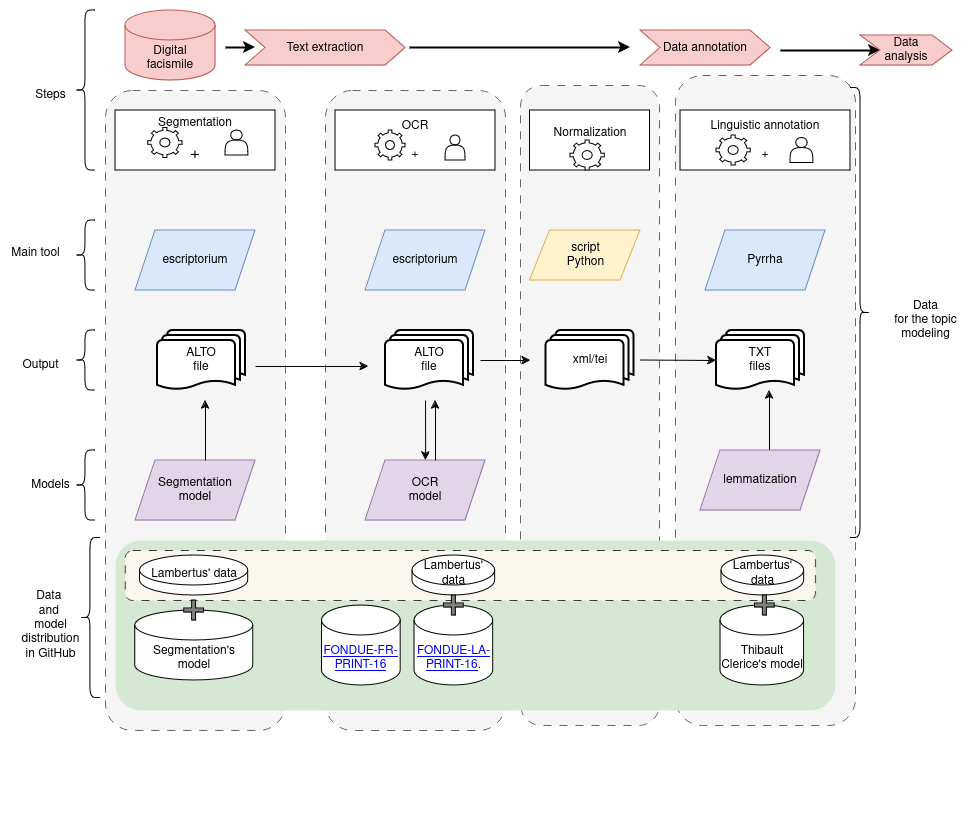
\includegraphics[width=.85\linewidth]{images/pipeline_2.png}
    \vspace{-0.4cm}
    \caption{Schéma décrivant les 4 étapes principales du traitement des données: la segmentation (\S~\ref{sec:Segmentation}), l'ATR (\S~\ref{sec:OCR}), la normalisation (\S~\ref{sec:normalisation}), l'annotation linguistique (\S~\ref{sec:Lemmatisation}).}
    \label{fig:pipeline}
    \vspace{-.4cm}
\end{figure}
%\FloatBarrier

\subsection{Analyse de mise en page}
\label{sec:Segmentation}
L'analyse de la page a été l'un des enjeux majeurs du projet. Pour ce faire, nous avons d'abord bénéficié d'un modèle de segmentation pour les imprimés français du  \textsc{xvi}\ieme{}~siècle \cite{humeau_2024_10602197,solfrini:hal-04555002}, puis du modèle de segmentation large développé dans le projet LaDaS~\cite{clerice:hal-04784161}.Pour finir, nous avons adapté le modèle LaDaS aux spécificités propres à la mise en page des commentaires exégétiques latins du \textsc{xvi}\ieme{}~siècle en fine-tunant un nouveau modèle \texttt{Layout-16th-Print-Lat}\cite{goy_2026_18492102} à partir de ce dernier\footnote{\url{https://github.com/ponteineptique/yaltai}}. 
\subsubsection{Données d'entraînement}

Nos données (tab.~\ref{tab:corpus}) sont distribuées dans un dépôt GitHub préparé selon les recommandations du projet \textit{HTR-United} \cite{chague_here_2023}: 
\textit{HTR-Corpus-A}\footnote{\url{https://github.com/16thExegesisDH/HTR-Corpus-A}}.
%\url{https://github.com/16thExegesisDH/HTR_1-Timotheus}
Pour garantir l'interopérabilité des données, nous avons recours au vocabulaire de SegmOnto~\cite{gabay2023b} tel que revu par le projet LADaS~\cite{clerice:hal-04784161} 
(fig.~\ref{fig:segmentation})\footnote{Le vocabulaire LADaS ayant évolué entre temps, notamment pour \texttt{-P-Continued} devenu \texttt{Continued}, le modèle a été produit en utilisant la première version, mais les données ont été corrigées dans le sens de la nouvelle version.}. Nos documents ne posent pas de problèmes particuliers en matière de mise en page. La préparation des données est faite avec eScriptorium~\cite{kiessling_escriptorium_2019}, dont l'Université de Genève héberge une instance~\cite{gabay2021}.

\subsubsection{Modélisation de la page}

 Notre objectif principal est une restructuration du document (texte vs paratexte, différentes parties et sous-parties) ainsi que la reconnaissance aussi automatique que possible des zones de titre intermédiaire (\texttt{MainZone-Head}) contenant très fréquemment les versets bibliques. Dans ce but, neuf types de zones ont été retenues (\S~\ref{appdx:ladas}).

\begin{figure}[!htb]
    \centering
    \begin{minipage}{.48\textwidth}
        \centering
    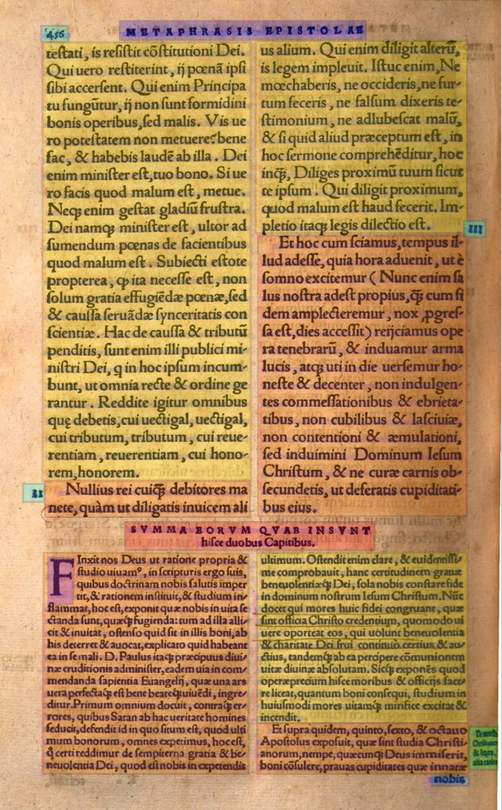
\includegraphics[height=8.7cm]{images/segmentation_ladas_2.png}
    \caption\small{Exemple de données d'entraînement.}
    \label{fig:segmentation}
    \end{minipage}%
    \hfill
    \begin{minipage}{0.48\textwidth}
        \centering
    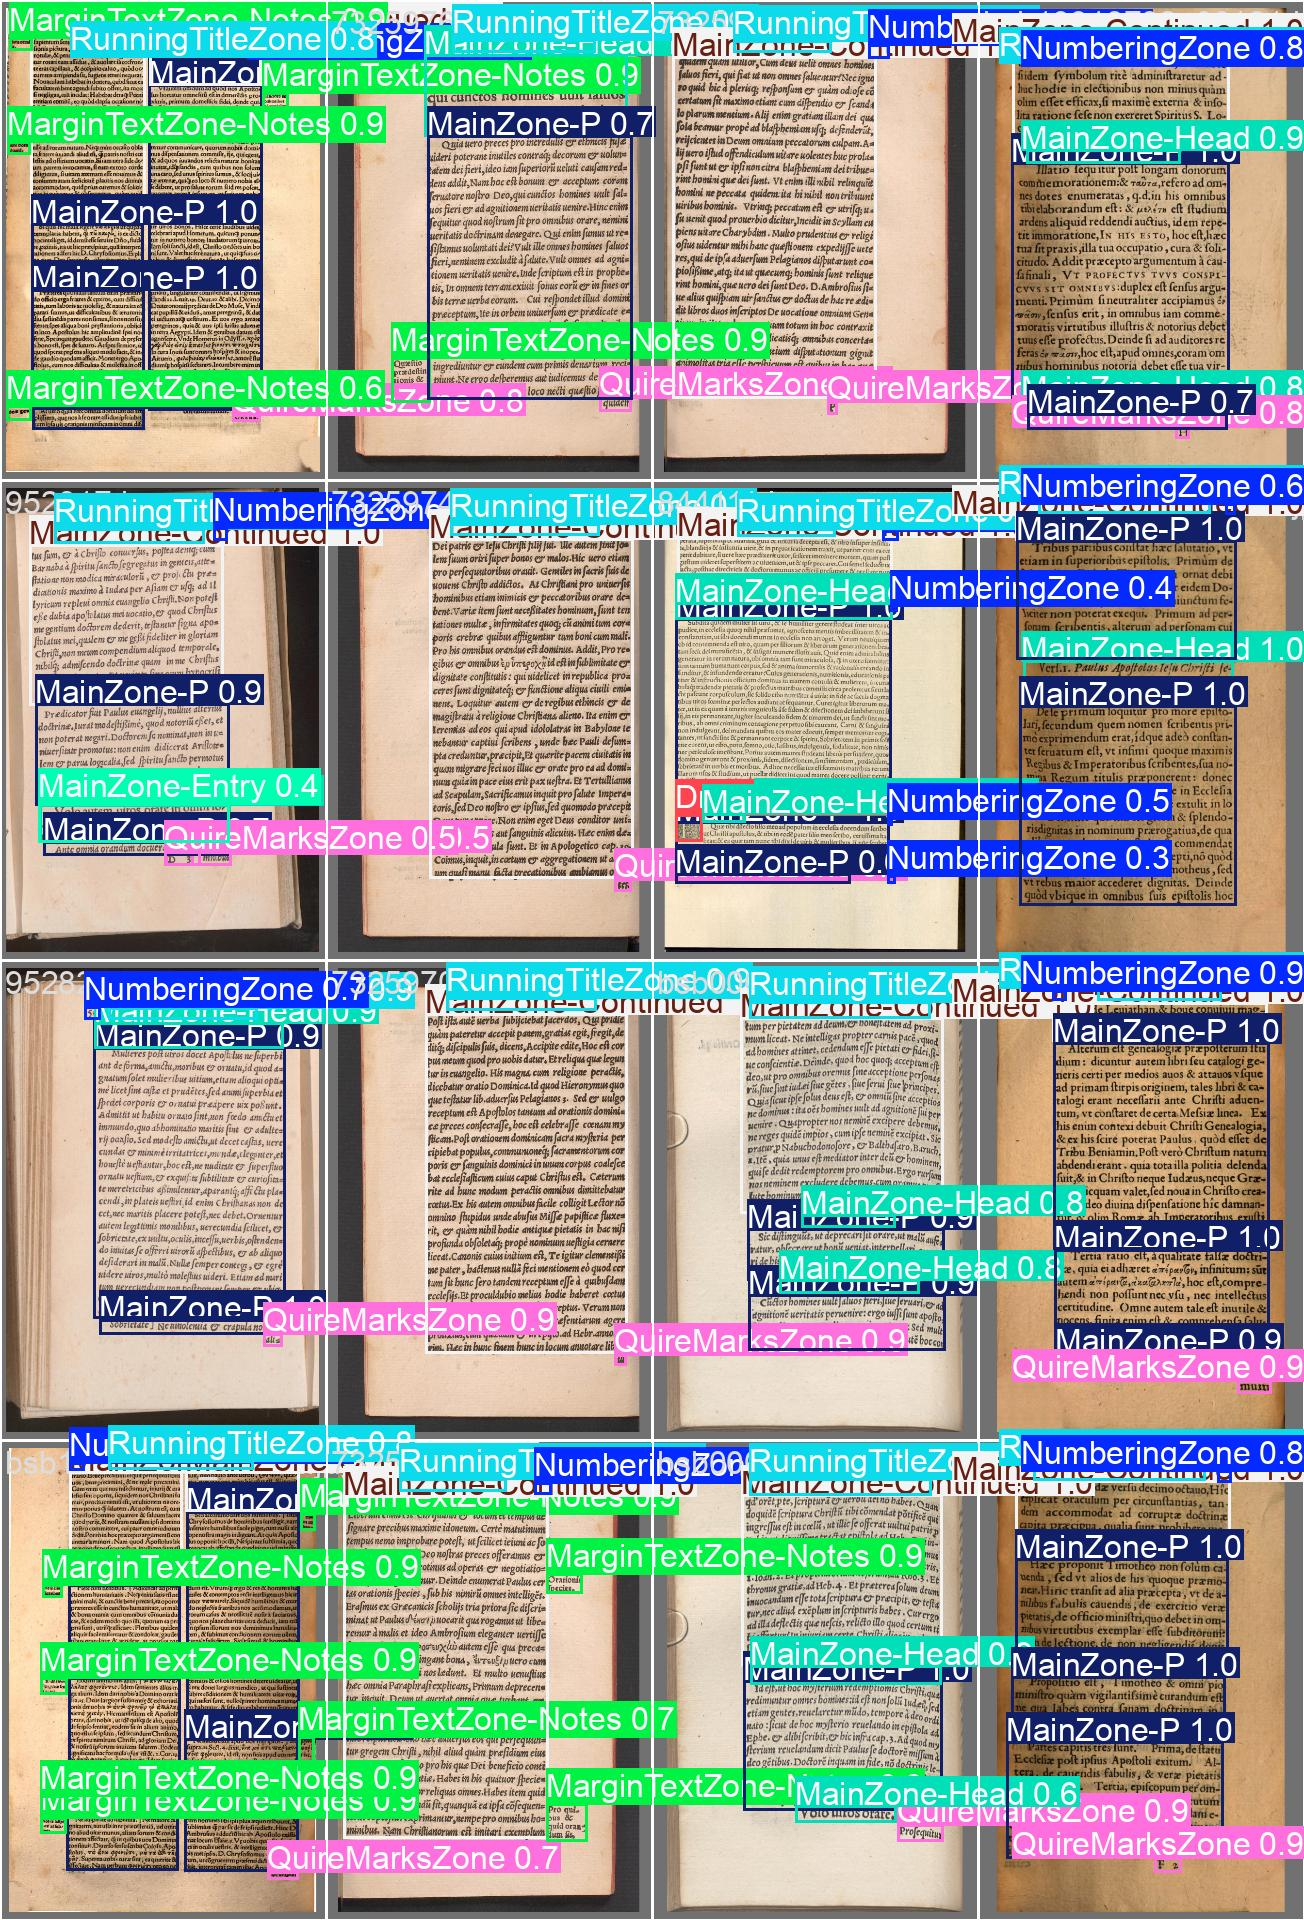
\includegraphics[height=8.7cm]{images/val_batch0_pred.jpg}
        \caption\small{Prédiction effectuées par notre modèle.}
        \label{fig:pred}
    \end{minipage}
    \vspace{-.5cm}
\end{figure}
\vspace{0.12cm}
\subsubsection{Entraînement et évaluation du modèle}
Le modèle de segmentation que nous avons entraîné a permis d'automatiser la tâche
d'annotation des images et ainsi d'accélérer le travail. En dépit de quelques
faiblesses persistantes, il présente les performances suivantes:

\begin{itemize}
    \item La matrice de confusion (fig.~\ref{fig:segm}) met en évidence une très bonne reconnaissance des éléments récurrents de la mise en page (\texttt{RunningTitle}, \texttt{MainZone-Continued}, \texttt{MainZone-P}, \texttt{QuireMarksZone}, \texttt{DropCapitalZone}, \texttt{MarginText-Notes}).
    \item~\texttt{MainZone-Head} est fréquemment correctement identifiée avec un score de 0{,}88, marquant une amélioration notable par rapport au modèle LaDaS, qui, dans le cas de nos imprimés, la confondait avec d’autres zones ou ne la détectait pas.
    \item La principale faiblesse du modèle concerne la \texttt{NumberingZone}. En raison de son ambiguité, la zone regroupe indistinctement la numérotation de page et la numérotation marginale du commentaire biblique (fig.~\ref{fig:segmentation}) ce qui engendre une confusion.
    \item Les éléments non reconnus relèvent majoritairement de données exclues du modèle (page de titre, index) ou insuffisamment représentées dans les données d’entraînement (par ex.~\texttt{GraphicZone}).
\end{itemize}

\begin{figure}[H]
    \centering
    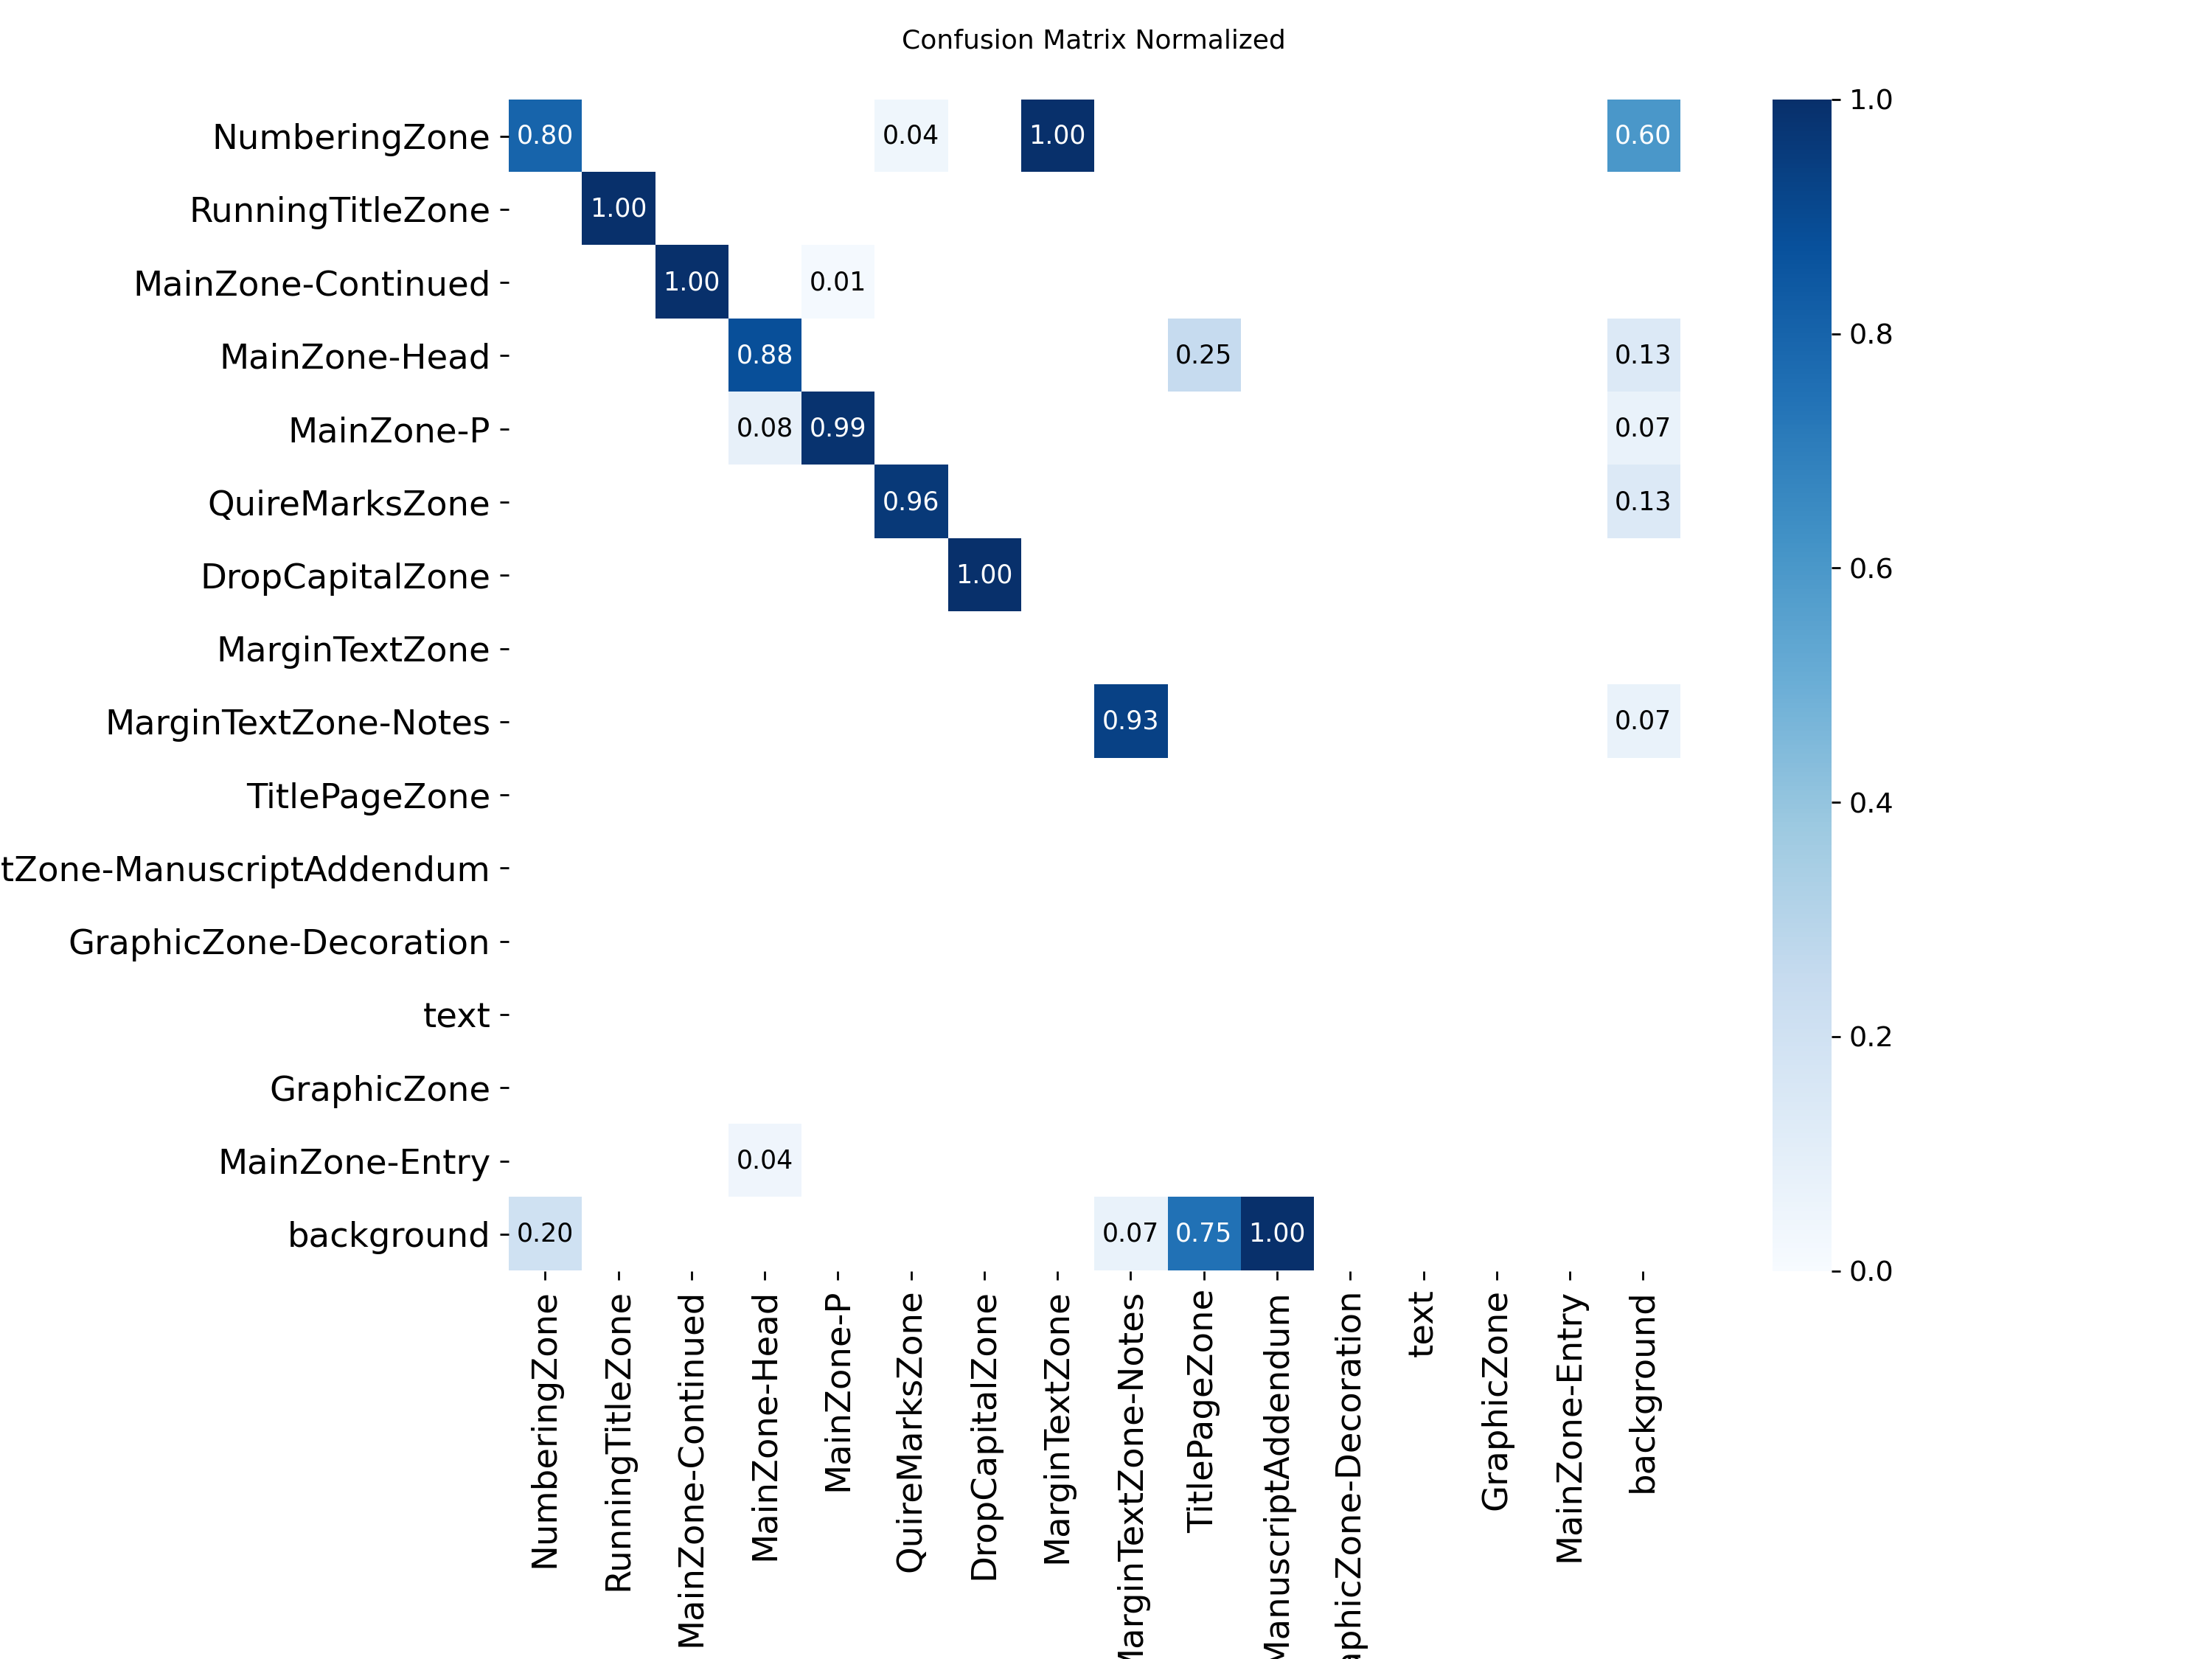
\includegraphics[width=0.65\textwidth]{images/confusion_matrix_normalized.png}
    \caption{\small Précision de la segmentation en fonction des zones.}
    \label{fig:segm}
\end{figure}

%L'OCR a été amélioré sur le modèle de Gallicorpora+\cite{pincheGallicorpora2022} destiné à travaillé sur des imprimés modernes (16e au 19e siècle) en langue française. Les données employées son amélioration proviennent de deux dépôts intégrés à la chaîne de traitement \href{https://htr-united.github.io/}{HTR-United} disponible sur l'espace GitHub de \href{https://github.com/FoNDUE-HTR?q=&type=all&language=&sort=}{~FONDUE} qui contiennent de documents imprimés au 16ème siècle en caractère roman \href{https://github.com/FoNDUE-HTR/FONDUE-FR-PRINT-16}{FONDUE-FR-PRINT-16} avec des documents en français et \href{https://github.com/FoNDUE-HTR/FONDUE-LA-PRINT-16}{FONDUE-LA-PRINT-16} avec des documents en latin (cf.Tableau\ref{dépôt-git-corpus}).


\subsection{Reconnaissance automatique de caractères}
\label{sec:OCR}
\begin{wrapfigure}{r}{0.6\textwidth}
    \centering\vspace{-.5cm}
    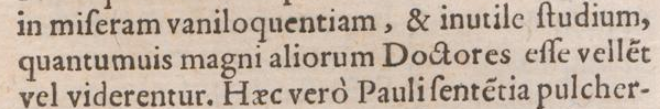
\includegraphics[width=.95\linewidth]{images/abréviations.png}
    \caption{Exemple d'abréviation latine (‹vell\~{e}t› et ‹sent\~{e}tia› avec un tilde sur le \textit{e} pour \textit{en}) et d'accent typique du néolatin (‹verò› doté d'un accent grave sur le \textit{o}.)
    \href{https://www.e-rara.ch/gep_g/content/zoom/2012928}{\textsc{Lamb.Dan.}\textit{~Ep. 1 Tim.} I,16}.}
    \label{fig:abréviations}
    \vspace{-.5cm}
\end{wrapfigure}
Au début de notre projet, nous avions à notre disposition le modèle du projet \textit{Gallicorpora} \cite{pinche_2022_7410529}, intégralement entraîné sur des données en français. Malheureusement, les premiers tests ont démontré d'importantes lacunes sur deux points: la transcription des abréviations et l'utilisation d'accents (fig.~\ref{fig:abréviations}).

\subsubsection{Données d'entraînement}

\begin{figure}[h]
    \centering
    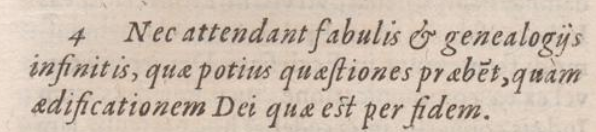
\includegraphics[width=.8\linewidth]{images/italique.png}
    \caption{L'italique est une typographie régulièrement employée pour distinguer visuellement le verset biblique de son commentaire. Cf.~par ex.~\href{https://www.e-rara.ch/gep_g/content/zoom/2012921}{\textsc{Lamb.Dan.}\textit{~Ep. 1 Tim.} I,9}.}
    \label{fig:italique}
\end{figure}
        
Si l'essentiel de nos données provient du commentaire de Lambert Daneau, nous avons recours à des échantillons provenant de pages prises de manière aléatoire dans les différents imprimés de notre corpus de travail (tab.~\ref{tab:corpus}).

Nos données comprennent, outre les documents que nous avons préparés, d'autres imprimés néolatins transcrits par Marie Jeannot-Tirole, provenant de son travail de thèse sur Ioannes Sapidus\footnote{\url{https://mariejeannot.gitpages.huma-num.fr/sapidus}.}. Les œuvres de ce dernier, des poèmes plutôt écrites en italique \cite{speyer:hal-02184237}, permettent d'augmenter la quantité de ce type de caractère, dont l'usage restait rare (fig.~\ref{fig:italique}) dans le corpus d'ATR que nous avions choisi.

Nos données ainsi que celles de M. Jeannot-Tirole, avec qui nous partageons les mêmes règles de transcription, sont distribuées dans un dépôt GitHub préparé selon les recommandations du projet \textit{HTR-United} \cite{chague_here_2023}: \texttt{FONDUE-LA-PRINT-16} \cite{gabay_fondue-la-print-16_2024}.

\vspace{0.3cm}
\begin{wrapfigure}{r}{0.5\textwidth}
    \centering\vspace{-.3cm}
    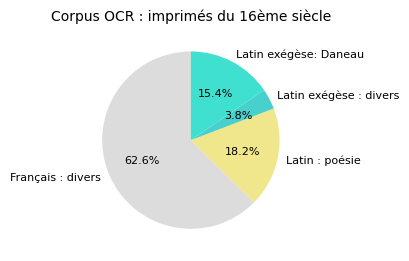
\includegraphics[width=.88\linewidth]{images/pie_chart.png}
    \caption{Origine de la vérité de terrain.}
    \label{fig:pie_chart}
    \vspace{-1cm}
\end{wrapfigure}

 Afin d'augmenter la quantité de données, nous avons aussi eu recours à des données provenant d'imprimés en langue française \cite{gabay_fondue-fr-print-16_2024}, obéissant également aux mêmes règles de transcription que les nôtres. Ce \textit{dataset} représente environ le tiers du total des données pour le \textsc{xvi}\ieme{}~s. (fig.~\ref{fig:pie_chart}).
\vspace{0.5cm}
\subsubsection{Règles de transcription}

Les règles de transcription présentées dans le projet CREMMA \cite{clericeCREMMAMediiAevi2023} couvrent l'essentiel des cas complexes. On y trouve en effet des recommandations pour les abréviations du latin médiéval, dont le système néolatin est une simplification. En dehors du phénomène d'accentuation, le néolatin ne présente donc pas de graphie nouvelle par rapport à celles des manuscrits médiévaux. Le seul caractère ajouté à notre transcription est ainsi le pied de mouche que les imprimeurs emploient pour indiquer les débuts des cahiers. On gardera à l'esprit qu'un corpus plus large donnera certainement à voir d'autres de ces signes typographiques.

\begin{figure}[htp]
    \centering
    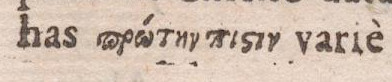
\includegraphics[width=.6\linewidth]{images/greek_alphabet.jpg}
    \caption{Exemple d'un passage en grec transcrit sans ligature, transcrit \textit{has πρώτην πιστιν variè}.}
    \label{fig:grec}
\end{figure}

Plus épineuse est la question des langues étrangères, comme le grec et l'hébreu, qui font en effet leur apparition dans les commentaires bibliques du \textsc{xvi}\ieme{} siècle. Dans le cas des commentaires pauliniens, l'hébreu est employé de manière anecdotique, il n'a donc pas été considéré dans cette étude. En revanche, les exégètes citent fréquemment le vocabulaire du texte source des épîtres: le grec. La transcription de cette seconde langue revêt donc un intérêt particulier pour la compréhension du propos du commentaire. Or, le grec des imprimés se décline à travers un système de ligature complexe \cite{wallace1923ligatures} qui nécessiterait à lui seul l'entraînement d'un modèle. Pour des raisons d'efficacité, il a été décidé de ne pas tenir compte de ces ligatures.

\subsubsection{Entraînement et évaluation du modèle}
    
Nous entraînons et évaluons trois modèles différents avec Kraken \cite{kraken}.
\vspace{0.3cm}
\begin{itemize}
    \item \texttt{Gallicorpora+}\footnote{\href{https://doi.org/10.5281/zenodo.7410529}{Modèle de Gallicorpora+}.} le modèle entraîné sur des imprimés anciens pour le projet \texttt{Gallicorpora}, qui n'a pas vu de vérité de terrain en (néo)latin;
    \item \texttt{gallicorpora\_ajuste}\cite{goy_2024_19218113} : version ajustée de \texttt{Gallicorpora+} sur les données du \textsc{xvi}\ieme{}~s. précédemment décrites;
    %\item \texttt{Model\_90}\footnote{\href{ https://github.com/FourbeFlo/OCR_test/releases/download/ml.model/lambertus_test_mai_best.mlmodel}{ modèle Model\_90}} : même configuration que \texttt{Model\_100}, moins 10\% des données du du \textsc{xvi}\ieme{}~s. pour évaluer notre marge de progression;
    \item \texttt{catmusPrint\_ajuste}: version ajustée du modèle CATMuS \textit{print} \cite{gabay:hal-04557457} sur les données du \textsc{xvi}\ieme{}~s. précédemment décrites et des données du \textsc{xvii}\ieme{}~s. \cite{gabay_2024_11526040}\footnote{Modèle entraîné par S.~Gabay, Th.~Clérice, et al. \cite{gabay_clerice_2024}.}.
\end{itemize}
\vspace{0.3cm}
Pour évaluer ces modèles, nous utilisons un double corpus hors domaine décrit dans le tab.~\ref{tab:outOfDomain}. Nous utilisons deux jeux de données différents: le premier contient des extraits de documents très proches de notre corpus de travail (test 1: commentaires pauliniens), et le second un document qui est toujours un commentaire biblique, mais dont le thème et la facture sont différents (test 2: commentaires bibliques).

\begin{table}[H]
    \centering
        \begin{tabular}{l|l|c c c c|}
        \toprule
        \textbf{Corpus} & \textbf{Métrique}  & \texttt{Gallicopora}  & \texttt{gallicorpora\_ajuste} & \texttt{catmusPrint\_ajuste} \\
        \midrule
        \multirow{2}{*}{\textbf{Test 1}} 
        & Acc & 97.95 & 98.96 & \textbf{99.14}\\
        & WAcc & 88.32 & 93.06 & \textbf{94.51}\\
        \hline
        \multirow{2}{*}{\textbf{Test 1+2}} 
        & Acc & 97.39 & 98.56 & \textbf{98.95}\\
        & WAcc & 86.19 & 91.11 & \textbf{93.35}\\
        \bottomrule
        \end{tabular}
        \caption{Résultats des 3 modèles sur les deux jeux de test. Les meilleurs résultats sont indiqués en gras. Le calcul de la WAcc est fait avec~\href{https://github.com/FoNDUE-HTR/kamiCLI}{kamiCLI}.}
        \label{tab:wide_table}
    \end{table}

\vspace{0.3cm}
\begin{wraptable}{r}{0.5\textwidth}
    \centering\footnotesize\vspace{-.6cm}
    \resizebox{\linewidth}{!}{
    \begin{tabular}{l l c c}
        \toprule
        \textbf{Corpus} & \textbf{Cote} & \textbf{Pages} & \textbf{Lines} \\
        \midrule
        \multirow{4}{*}{\textbf{Test 1}} 
        & \href{https://doi.org/10.3931/e-rara-6338}{BGE Cti 1753 BGE S 22877}  & 2 & 72 \\ 
        & \href{https://doi.org/10.3931/e-rara-19975}{BCUL, AZ 8515 (4)} & 2 & 61 \\ 
        & \href{https://doi.org/10.3931/e-rara-8160}{ZB, C 283,2} & 2 & 51 \\ 
        \midrule
        \textbf{Test 2} 
         & \href{https://doi.org/10.3931/e-rara-75521}{BGE Cta 3110 (1)} &   &  \\
         & \href{https://doi.org/10.3931/e-rara-75521}{BGE Bb 1049 (1)} & 2 & 88  \\
        \midrule
        \textbf{Total} &  & \textbf{8} & \textbf{272} \\
        \bottomrule
    \end{tabular}
    }
    \caption{Corpus de données \textit{out-of-domain} pour le test d'ATR.}
    \label{tab:outOfDomain}
\end{wraptable}

Sans grande surprise, si les résultats sont satisfaisants pour les trois modèles, le modèle \texttt{catmusPrint\_ajuste} obtient les meilleurs scores, notamment avec l'ajout du jeu de test 2. Si le gain au niveau de la \textit{character accuracy} (CAcc) est relativement modeste, celui au niveau de la \textit{word accuracy} (WAcc) est plus net, justifiant l'entraînement de nouveaux modèles en dépit de scores \textit{a priori} corrects au premier abord.

\subsection{Normalisation linguistique}
\label{sec:normalisation}
De récentes études ont démontré la supériorité des approches neuronales pour la normalisation linguistique~\cite{gabay-barrault-2020-traduction,bawden:hal-03540226}. Les imprimés en néolatin présentent cependant une relative stabilité tant dans leurs pratiques graphiques que dans le système abréviatif: nous avons donc choisi une approche à base de règles, en utilisant des expressions régulières\footnote{Le script est disponible en ligne:\url{https://github.com/16thExegesisDH/PipeLineThm/tree/main/PYTHON/normalisation}
.}.

\subsubsection{Méthode}

La normalisation est ici comprise comme un alignement de la transcription sur les normes régissant le latin classique, la plupart des outils disponibles étant prévus pour traiter ce type de texte. Elle concerne en particulier : 

\begin{itemize}
    \item le système abréviatif : résolution des tildes…;
    \item les accents et les cédilles: suppression des accents typiques des imprimés en néolatins…; 
    %\item les lettres ramistes: rétablissement du ‹u› pour le son consonne; % ce n'est plus le cas (Ueli's wishes) 
    \item les ligatures: passage de ‹æ›/‹e› cédillé à ‹ae›, de ‹œ› à ‹oe›…
    \item les allographes: passage du \textit{s} long (‹ſ›) au \textit{s} rond;
\end{itemize}

Notre script permet un lissage de la variation graphique par rapport au latin classique, mais pas de corriger des évolutions plus lourdes, du type \textit{auctor} (latin classique) $\to$ \textit{author} (néolatin) ou \textit{saeculum} (latin classique) $\to$ \textit{seclum} ou \textit{seculum} (néolatin).

\subsubsection{Résultats}

La normalisation est stockée dans une balise \texttt{<reg>} à côté du texte extrait par le moteur ATR, conservé dans un \texttt{<orig>}.

\begin{minted}[
  linenos,
  xleftmargin=2em,
  breaklines,
  fontsize=\footnotesize
]{xml}
<lb corresp="#f2013098_line_26_ligne_8"/>
    choice>
        <orig>affectum animi. Sanæ, doctrinæ opponitur tum</orig>
        <reg type="normalized">affectum animi. Sanae, doctrinae opponitur tum</reg>
    </choice>
<lb corresp="#f2013098_line_27_ligne_9"/>
    <choice>
        <orig>quod ſuprà dixit eam doctrinã Diabolicam eſſe:</orig>
        <reg type="normalized">quod supra dixit eam doctrinam Diabolicam esse:</reg>
    </choice>
\end{minted}

\subsection{Annotation linguistique}
\label{sec:Lemmatisation}
\begin{wraptable}{r}{0.4\textwidth}
    \centering\small\vspace{-.4cm}
    \begin{tabular}{l l c c}
        \toprule
        \textbf{Parties} & \textbf{Pages} & \textbf{Lemmes} \\
        \midrule
        Préface & 24 & 4 781 \\
        Chapitre I & 37 & 9 477 \\
        Chapitre II & 15 & 4 071 \\
        \toprule
        \textbf{total} & 76 & 18 329 \\
        \bottomrule
    \end{tabular}
    \caption{Corpus pour l'annotation linguistique.}
    \label{tab:annotation}
    \vspace{-1cm}
\end{wraptable}
La préparation des données pour entraîner les modèles d'annotation linguistique a été effectuée avec \textit{Pyrrha} \cite{clerice_building_2022}.

\subsubsection{Données d'entraînement}
Nous avons contrôlé 18~329 tokens\footnote{\url{https://github.com/FourbeFlo/Lemmatization/blob/main/Lambertus_corrected.tsv}.}, tous tirés des deux premiers chapitres du commentaire de Lambert Danneau (\S\ref{tab:corpus}), soit environ septante pages situées au début de l'œuvre (tab.~\ref{tab:annotation}). 

\subsubsection{Référentiel, cas particuliers}
Les lemmes proviennent du dictionnaire de Forcellini \cite{forcellini1940}, afin de de conserver une interopérabilité avec le travail de Th.~Clérice \cite{cléri2022}. L'utilisation de \textit{Pyrrha} permet de garantir une qualité minimale de l'annotation (contrôle des valeurs possibles en POS, liste de lemmes possibles…). 

La qualité de la prédiction proposée par le modèle LASLA distribué par \textit{Pie extended} \cite{thibault_clerice_2020_3883590} est globalement de grande qualité. L'essentiel des problèmes concerne:
\begin{itemize}
\item le vocabulaire propre au latin chrétien et néolatin: \textit{papista}, \textit{excommunicatio}…;
\item les noms bibliques: \textit{Ezechias}…; 
\item les noms des penseurs chrétiens: \textit{Augustinus}…; 
\item les variantes néolatines de mots classiques:  \textit{author}, \textit{seculus}…; 
\item Les abréviations des différents livres bibliques: \textit{Apocalyp} pour \textit{Apocalypsis}…
\end{itemize}
Les abréviations de livres bibliques sont le problème majeur de notre corpus exégétique, car elles ne sont pas standardisées. Par exemple, le nom de l'Évangile de Matthieu est abrégé de trois manières différentes : ‹Math›, ‹Matth›, ‹Matt›. Nous avons choisi de regrouper ces trois tokens derrière le lemme \textit{Matthaeus} tel que l'orthographie le dictionnaire de Forcellini. À chaque fois que nous rencontrons une abréviation biblique, nous en gardons la trace dans un fichier csv, ce qui nous permet de tenir à jour leur liste à compléter avec l'avancée du projet\footnote{\url{https://github.com/FourbeFlo/Lemmatization/blob/main/dictionaries\%20and\%20abbreviations/livre-biblique.csv}.
}.

\subsubsection{Résultat}

Les données d'entraînement pour un méga modèle n'étant pas publiques, nous nous sommes tournés vers CLTK (Classical Latin Toolkits)\cite{johnson-etal-2021-classical}, une bibliothèque Python de NLP pour les langues pré-modernes qui intègre notamment les modèles neuronaux de Stanza \cite{qi2020stanzapythonnaturallanguage}\cite{burns2023latincysynthetictrainedpipelines} pour l’annotation linguistique. Bien que n'ayant pas la précision que l'on pourrait espérer avec un annotateur linguistique entraîné spécifiquement pour notre corpus, la grande variété de textes latins intégrés par CLTK permet des résultats satisfaisants lors de la lemmatisation des textes comme le démontre les premiers essais de \textit{topic modeling} (fig.~\ref{fig:topic}). % préciser que s'appuie sur le latin clasique, médiéval et néolatin. 

\begin{figure}[htp]
    \centering
    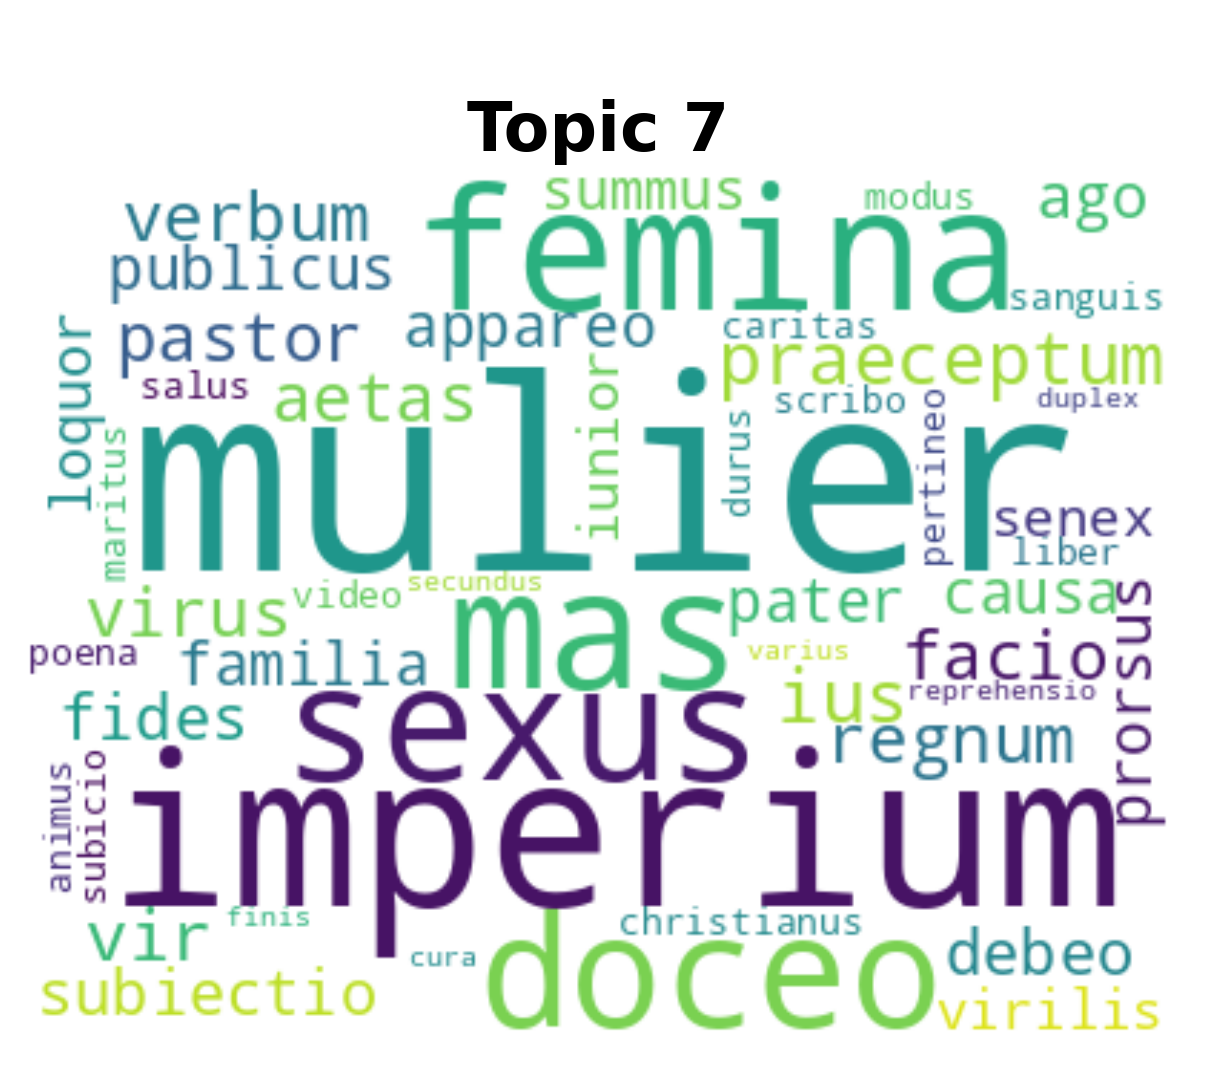
\includegraphics[width=0.5\linewidth]{images/topic_wordclouds_7_mulier.png}
    \caption{Résultat de topic modeling effectué sur ~\href{https://www.e-rara.ch/gep_g/content/zoom/2012921}{\textsc{Lamb.Dan.}\textit{~Ep. 1 Tim.}}; le \textit{Topic} 7 concernant la notion de femme : \textit{mulier}.}
    \label{fig:topic}
\end{figure}

\section{Conclusion}
Le travail présenté constitue une description de notre chaîne de traitement, laquelle pourrait sans doute être encore améliorée, notamment par l’ajout de nouvelles données \textit{gold} pour renforcer la performance des différents modèles. Le corpus définitif n’étant pas encore entièrement stabilisé, il est possible que nous rencontrions à l’avenir des cas présentant des variations de mise en page, de typographie ou d’autres caractéristiques absentes des données actuellement disponibles. Les données que nous avons préparées ont néanmoins déjà permis de consolider certains modèles, tels que ceux dédiés à l’analyse de mise en page ou à l’ATR, et continueront de jouer un rôle essentiel dans des tâches comme l’annotation linguistique. En ce sens, elles ont contribué à faciliter les études computationnelles sur le néolatin, une langue encore insuffisamment explorée sur le plan numérique.

\section*{Financement}

Les recherches ont été menées dans le cadre du projet \textit{Paulusauslegung des 16. Jahrhunderts} (FNS \href{https://data.snf.ch/grants/grant/207696}{\underline{n° 207696}}).



%En parallèle de la constitution du corpus, nous avons commencé à explorer son contenu de manière approfondie. Nous prévoyons notamment d’utiliser la modélisation de sujets, une approche qui permettra d’identifier les thématiques dominantes dans les différents commentaires et de suivre leur évolution au fil du temps. Dans la dernière phase du projet, il sera nécessaire de publier l’ensemble du corpus via une bibliothèque numérique, afin de rendre les documents accessibles tant pour la lecture que pour leur exploitation dans le cadre d’études de corpus. Une première ébauche de cette bibliothèque est disponible en ligne\footnote{\url{https://16thexegesisdh.github.io/ReformingPaul/index.html}}. L'interface devrait fournir à la fois l'accès aux textes exploités et des outils pour leurs analyses digitales. Cette démarche contribuera à une meilleure diffusion des données et à une compréhension plus fine des dynamiques thématiques qu’elles révèlent.
%\clearpage
% Imprime la bibliographie à la fin. Gardez cette ligne après le texte
% principal de votre article et avant une annexe.
\printbibliography

% Vous pouvez inclure une annexe en utilisant la commande suivante
\appendix

\section{Nommage des zones}
\label{appdx:ladas}

\vspace{0.1cm}
\begin{itemize}
    \item \texttt{RunningTitleZone} pour le titre courant en haut de page;
    \item \texttt{MarginTextZone-Notes} pour les commentaires marginaux;
    \item \texttt{NumberingZone} pour la numérotation (pagination ou foliotation);
    \item \texttt{QuireMarksZone} pour l'organisation des cahiers;
    \item \texttt{GraphicZone} pour toutes les décorations (illustrations, ornementation…);
    \item \texttt{DropCapitalZone} pour les lettrines en début de partie;
    \item \texttt{MainZone-P} pour un paragraphe;
    \item \texttt{MainZone-Continued} pour la suite d'un paragraphe interrompu ;
    \item  \texttt{MainZone-Head} pour le titre intermédiaire et les versets bibliques, lorsqu'ils sont mis en valeur par la mise en page
\end{itemize}
\vspace{0.1cm}
Les lignes ont été classées en deux catégories:
\vspace{0.1cm}
\begin{itemize}
    \item \texttt{HeadingLine} continent tout les éléments de titre, sous-titre, etc.;
    \item \texttt{DefaultLine} décrit la ligne par défaut.
\end{itemize}

%Des annexes facultatives peuvent être ajoutées après la section des références. 

\end{document}